% Author: Izaak Neutelings (July 2021)
% Description: B tagging of a jet
% Inspiration:
%  Nazar Bartosik, https://commons.wikimedia.org/wiki/File:B-tagging_diagram.png
%  https://indico.cern.ch/event/687697/contributions/2825792/attachments/1579225/2494980/bjet_tagging_via_trackIP.pdf
%  B tagging algorithm at ATLAS: https://arxiv.org/abs/1711.08811
%  B tagging algorithm at CMS: https://arxiv.org/abs/1712.07158
\documentclass[border=3pt,tikz]{standalone}
\usepackage{amsmath}
%\usepackage{physics}
\usepackage{xcolor}
\usepackage[outline]{contour} % glow around text
\usetikzlibrary{calc}
\usetikzlibrary{math} % for \tikzmath
\usetikzlibrary{arrows.meta}
\usetikzlibrary{decorations.pathreplacing} % for curly braces
\contourlength{0.5pt}
\tikzset{>=latex} % for LaTeX arrow head

\colorlet{myred}{red!80!black}
\colorlet{myblue}{blue!75!black}
\colorlet{mydarkblue}{blue!40!black}
\colorlet{mygreen}{green!50!black}
\colorlet{mylightgreen}{green!70!black}
\colorlet{mydarkgreen}{green!20!black}
\colorlet{myorange}{orange!80!red!85!black}
\tikzstyle{track}=[->,line width=0.65,blue!40!black]
\tikzstyle{beam}=[myorange!30,dashed,line width=0.7,line cap=round]
\tikzstyle{mydashed}=[dash pattern=on 2pt off 2.5pt,line cap=round]
\tikzstyle{myshortdashed}=[dash pattern=on 1.5pt off 2pt,line cap=round]
\tikzstyle{measure}=[{Latex[length=2.2,width=2.2]}-{Latex[length=2.2,width=2.2]}]

\newcommand\jetcone[6][blue]{{
  \pgfmathanglebetweenpoints{\pgfpointanchor{#2}{center}}{\pgfpointanchor{#3}{center}}
  \edef\ang{#4/2}
  \edef\e{#5}
  \edef\vang{\pgfmathresult} % angle of vector OV
  \tikzmath{
    coordinate \C;
    \C = (#2)-(#3);
    \x = veclen(\Cx,\Cy)*\e*sin(\ang)^2; % x coordinate P
    \y = tan(\ang)*(veclen(\Cx,\Cy)-\x); % y coordinate P
    \a = veclen(\Cx,\Cy)*sqrt(\e)*sin(\ang); % vertical radius
    \b = veclen(\Cx,\Cy)*tan(\ang)*sqrt(1-\e*sin(\ang)^2); % horizontal radius
    \angb = acos(sqrt(\e)*sin(\ang)); % angle of P in ellipse
  }
  \coordinate (tmpL) at ($(#3)-(\vang:\x pt)+(\vang+90:\y pt)$); % tangency
  \coordinate (tmpO) at ($(#2)+(\vang:0.01)$); % origin shifted
  \coordinate (tmpO') at ($(#2)+(\vang:0.02)$); % origin shifted 2
  \fill[white,rotate=\vang] % fill background white
    (tmpL) arc(180-\angb:180+\angb:{\a pt} and {\b pt})
    -- (tmpO) -- cycle;
  \draw[thin,#1!40!black,rotate=\vang, %,fill=#1!50!black!80
    top color=#1!45!black!60,bottom color=#1!60!black!50,shading angle=\vang]
    (#3) ellipse({\a pt} and {\b pt});
  \begin{scope}[rotate=\vang] % already rotate for easy adjustments to full cone
    #6 % extra tracks
  \end{scope}
  \draw[thin,#1!30!black,rotate=\vang,
  top color=#1!90!black!80,bottom color=#1!25!black!90,shading angle=\vang,fill opacity=0.3]
    (tmpL) arc(180-\angb:180+\angb:{\a pt} and {\b pt})
    -- (tmpO) -- cycle;
}}

\newcommand\rightAngle[4]{
  \pgfmathanglebetweenpoints{\pgfpointanchor{#2}{center}}{\pgfpointanchor{#1}{center}}
  \pgfmathsetmacro\tmpx{\pgfmathresult}
  \pgfmathanglebetweenpoints{\pgfpointanchor{#2}{center}}{\pgfpointanchor{#3}{center}}
  \pgfmathsetmacro\tmpy{\pgfmathresult}
  \draw[green!20!black] (#2)++(\tmpx:#4) --++ (\tmpy:#4) --++ (\tmpx+180:#4);
}


\begin{document}


% B TAGGING
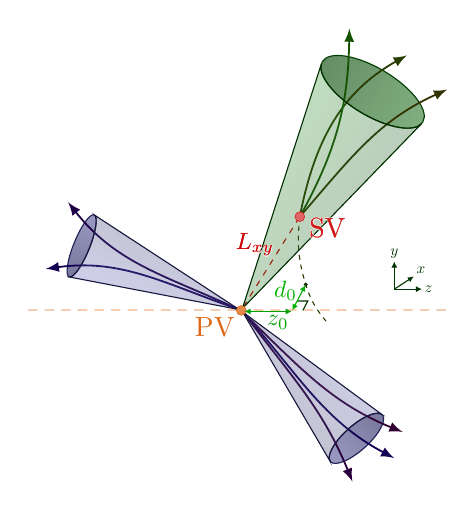
\begin{tikzpicture}[scale=2.7]


  \def\R{1.0}
  \coordinate (O) at (0,0); % primary vertex
  \coordinate (BJ) at ( 59:1.20*\R); % b jet 1
  \coordinate (SV) at ( 58:0.52*\R); % secondary vertex
  \coordinate (J1) at (158:0.81*\R); % q jet 1
  \coordinate (J2) at (-48:0.81*\R); % q jet 2
  \coordinate (IPz) at (0.24,0); % project (IP) onto beam axis
  
  % BEAM (behind)
  \draw[beam]
    (-1,0) -- (0,0) coordinate(X);
  
  % JETS
  \jetcone[myblue!70!white]{O}{J1}{22}{0.06}{
    \draw[track,blue!80!red!40!black] (tmpO') to[out=3,in=-150] (10:0.94*\R);
    \draw[track,blue!70!red!40!black] (tmpO') to[out=-3,in=150] (-10:0.96*\R);
  }
  \jetcone[myblue!70!white]{O}{J2}{23}{0.13}{
    \draw[track,blue!50!red!40!black] (tmpO') to[out=4,in=-154] (11:0.95*\R);
    \draw[track,blue!80!red!40!black] (tmpO') to[out=0,in=-160] (4:1.00*\R);
    \draw[track,blue!60!red!40!black] (tmpO') to[out=-5,in=160] (-9:0.96*\R);
  }
  \jetcone[green!60!black]{O}{BJ}{26}{0.17}{
    \draw[track,green!60!red!40!black] (SV) to[out=20,in=-210] (-2:1.43*\R);
    \draw[track,green!80!red!40!black] (SV) to[out=2,in=-150] (10:1.42*\R);
    \draw[track,green!50!red!40!black] (SV) to[out=-10,in=145] (-12:1.42*\R);
    \draw[line width=0.5,green!60!red!40!black,myshortdashed,line width=0.4]
      (SV) to[out=-155,in=48]++ (-144:0.32*\R) coordinate(IP)
           to[out=228,in=70]++ (240:0.20*\R);
    \draw[mydashed,myred] (tmpO') -- (SV);
  }
  \path (O) -- (SV)
    %node[pos=0.8,left=0,myred,opacity=0.5] {\contour{white}{B}}
    %node[pos=0.8,left=0,myred] {B} % B hadron
    node[pos=0.7,left=0,myred,scale=0.85,opacity=0.7] {\contour{white}{$L_{xy}$}}
    node[pos=0.7,left=0,myred,scale=0.85] {$L_{xy}$}; % SV distance
  \draw[beam] % beam (behind)
    (0.96,0) coordinate(X) -- (O);
  
  % VERTICES
  \draw[myorange!90,fill=myorange!70,very thin] % primary vertex
    (O) circle(0.023) node[below left=-1] {PV};
  \draw[myred!90,fill=myred!60,very thin] % secondary vertex
    (SV) circle(0.023)
    node[below=4,right=0,opacity=0.7] {\contour{white}{SV}}
    node[below=4,right=0] {SV};
  
  % POINT OF CLOSEST APPROACH
  %\coordinate (IPz) at ($(O)!(IP)!(X)$); % project (IP) onto beam axis
  \rightAngle{X}{IPz}{IP}{0.05}
  \draw[green!70!red!20!black,fill=green!70!red!40!black,very thin]
    (IP) circle(0.008); % node[below right=-1] {\contour{white}{DCA}};
  \draw[mylightgreen,measure,shorten <=0.05,shorten >=0.3]
    (IPz) -- (IP)
    node[pos=0.75,left=-1,scale=0.85] {$d_0$};
  \draw[mylightgreen!90!black,measure,shorten <=1.2,shorten >=0.2]
    (0,-0.005) --++ (IPz)
    node[pos=0.72,below=-1.5,scale=0.85] {$z_0$};
  
  % COORDINATE AXIS
  \draw[mydarkgreen,measure]
    (0.85,0.1) node[right=-1,scale=0.55] {$z$} --++ (-0.13,0) coordinate(O')
    --++ (0,0.13) node[above=-1,scale=0.55] {$y$};
  \draw[mydarkgreen,-{Latex[length=2.2,width=2]}]
    (O') --++ (33:0.11) node[above right=-1,scale=0.55] {$x$};
  
\end{tikzpicture}


% B TAGGING
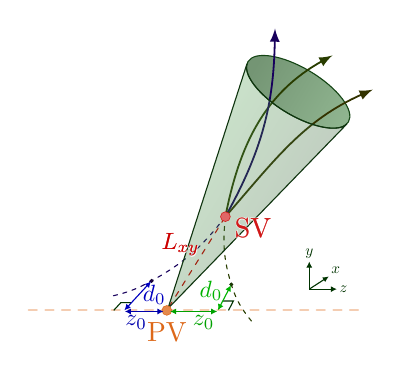
\begin{tikzpicture}[scale=2.7]
  \def\R{1.0}
  \coordinate (O) at (0,0); % primary vertex
  \coordinate (BJ) at ( 59:1.20*\R); % b jet 1
  \coordinate (SV) at ( 58:0.52*\R); % secondary vertex
  \coordinate (J1) at (158:0.81*\R); % q jet 1
  \coordinate (J2) at (-48:0.81*\R); % q jet 2
  \coordinate (IPz) at (0.24,0); % project (IP) onto beam axis
  \coordinate (IP2z) at (-0.20,0); % project (IP) onto beam axis
  
  % BEAM (behind)
  \draw[beam]
    (-0.65,0) coordinate(-X) -- (0,0);
  
  % JET
  \jetcone[green!60!black!80!white]{O}{BJ}{26}{0.17}{
    \draw[track,green!60!red!40!black] (SV) to[out=20,in=-210] (-2:1.43*\R);
    \draw[track,blue!80!red!45!black] (SV) to[out=2,in=-150] (10:1.42*\R);
    \draw[track,green!50!red!40!black] (SV) to[out=-10,in=145] (-12:1.42*\R);
    \draw[line width=0.5,green!60!red!40!black,myshortdashed,line width=0.4] % right
      (SV) to[out=-155,in=48]++ (-144:0.32*\R) coordinate(IP)
           to[out=228,in=70]++ (240:0.20*\R);
    \draw[line width=0.5,blue!80!red!45!black,myshortdashed,line width=0.4] % left
      (SV) to[out=173,in=-30]++ (162:0.46*\R) coordinate(IP2)
           to[out=-210,in=-46]++ (-218:0.20*\R);
    \draw[mydashed,myred] (tmpO') -- (SV);
  }
  \path (O) -- (SV)
    node[pos=0.7,left=0,myred,scale=0.85,opacity=0.7] {\contour{white}{$L_{xy}$}}
    node[pos=0.7,left=0,myred,scale=0.85] {$L_{xy}$}; % SV distance
  \draw[beam] % beam (behind)
    (0.90,0) coordinate(X) -- (O);
  
  % VERTICES
  \draw[myorange!90,fill=myorange!70,very thin] % primary vertex
    (O) circle(0.023) node[below=1] {PV};
  \draw[myred!90,fill=myred!60,very thin] % secondary vertex
    (SV) circle(0.023)
    node[below=4,right=0,opacity=0.7] {\contour{white}{SV}}
    node[below=4,right=0] {SV};
  
  % POINT OF CLOSEST APPROACH 1 (right, green)
  \rightAngle{X}{IPz}{IP}{0.05}
  \draw[green!70!red!20!black,fill=green!70!red!40!black,very thin]
    (IP) circle(0.008);
  \draw[mylightgreen,measure,shorten <=0.05,shorten >=0.3]
    (IPz) -- (IP)
    node[pos=0.75,left=-1,scale=0.85] {$d_0$};
  \draw[mylightgreen!90!black,measure,shorten <=1.2,shorten >=0.2]
    (0,-0.005) --++ (IPz)
    node[pos=0.72,below=-1.5,scale=0.85] {$z_0$};
  
  % POINT OF CLOSEST APPROACH 2 (left, blue)
  \rightAngle{-X}{IP2z}{IP2}{0.05}
  \draw[blue!70!red!20!black,fill=blue!70!red!45!black,very thin]
    (IP2) circle(0.008);
  \draw[myblue,measure,shorten <=0.05,shorten >=0.3]
    (IP2z) -- (IP2)
    node[pos=0.53,right=-1.5,scale=0.85] {$d_0$};
  \draw[myblue!90!black,measure,shorten <=1.2,shorten >=0.2]
    (0,-0.005) --++ (IP2z)
    node[pos=0.72,below=-1.5,scale=0.85] {$z_0$};
  
  % COORDINATE AXIS
  \draw[mydarkgreen,measure]
    (0.80,0.1) node[right=-1,scale=0.55] {$z$} --++ (-0.13,0) coordinate(O')
    --++ (0,0.13) node[above=-1,scale=0.55] {$y$};
  \draw[mydarkgreen,-{Latex[length=2.2,width=2]}]
    (O') --++ (33:0.11) node[above right=-1,scale=0.55] {$x$};
  
\end{tikzpicture}


\end{document}